In leading order we have to consider photon-gluon-fusion (PGF), that is
\begin{equation}
b(q) + \Pg(k_1) \rightarrow \PQ(p_1)+\PaQ(p_2),\quad b\in\{\Pggx,\PZx\}
\end{equation}
with two contributing diagrams depicted in figure \ref{fig:FeynLO}.
\begin{figure}[ht!]
\centering
\begin{subfigure}[t]{.4\textwidth}
	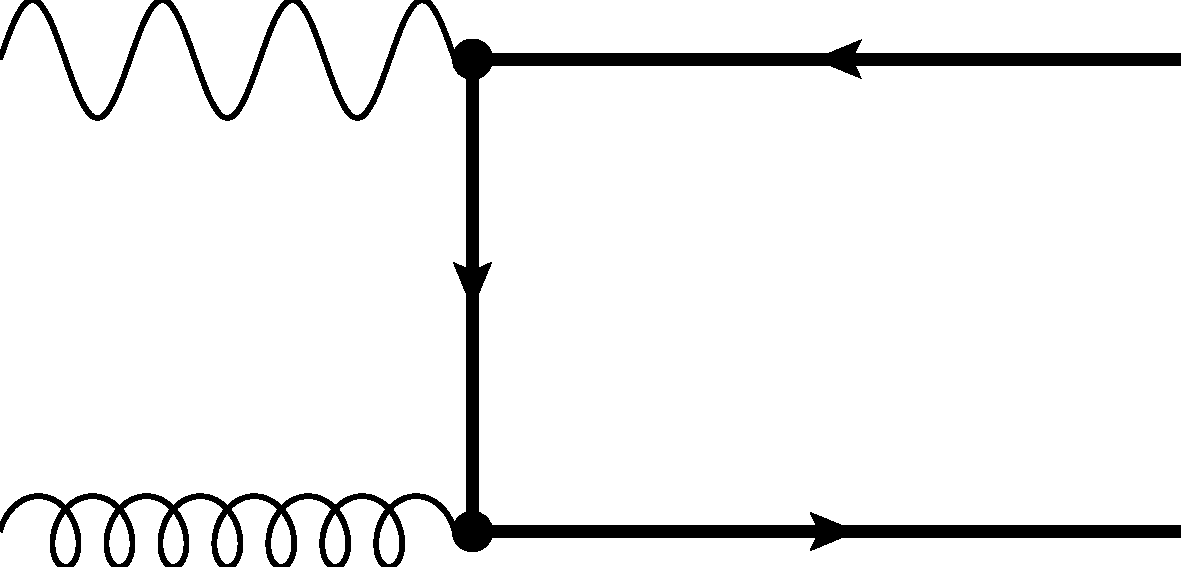
\includegraphics[width=\textwidth]{pyfeyn/lo-1}
	\caption{$i\varepsilon^{\mu}_{b}(q)\varepsilon^{\nu}_{\Pg}(k_1)\Md^{(0),1}_{\mu\nu}$}
\end{subfigure}\hspace{.15\textwidth}%
\begin{subfigure}[t]{.4\textwidth}
	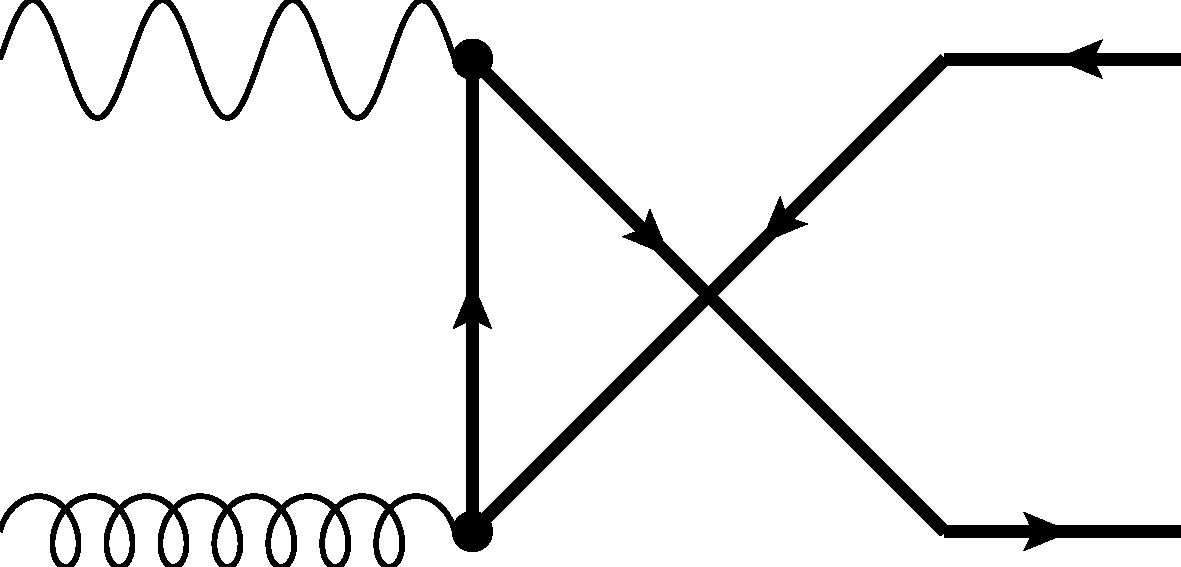
\includegraphics[width=\textwidth]{pyfeyn/lo-2}
	\caption{$i\varepsilon^{\mu}_{b}(q)\varepsilon^{\nu}_{\Pg}(k_1)\Md^{(0),2}_{\mu\nu}$}
\end{subfigure}
\caption{leading order Feynman diagrams}\label{fig:FeynLO}\fxerror{shift to appendix?}
\end{figure}

The result can then be written as
\begin{equation}
M_{\vec \kappa}^{(0)} = \hat {\mathcal P}_{\vec \kappa}^{b,\mu\mu'}\hat {\mathcal P}_{\kappa_2}^{\Pg,\nu\nu'}\sum_{j,j'=1}^2\Md^{(0),j}_{\mu\nu}\left(\Md^{(0),j'}_{\mu'\nu'}\right)^* = 8g^2\mu_D^{-\epsilon}e^2e_H^2 N_C C_F B_{\vec \kappa,\tQED}
\end{equation}
where $g$ and $e$ are the strong and electromagnetic coupling constants respectively, $\mu_D$ is an arbitray mass parameter introduced to keep the couplings dimensionless and $e_H$ is the magnitude of the heavy quark in units of $e$. Further $N_C=3$ corresponds to the gauge group $SU(N_C)$ and the color factor $C_F=(N_C^2-1)/(2N_C)$ refers to the second Casimir constant of the fundamental representation for the quarks. We then find:
\begin{align}
B_{\tVV,F_2,\tQED} &= \left[-1 - \frac{6q^2}{s'} - \frac{6q^4}{{s'}^2} + \frac{q^2(6m^2+s) +2m^2 s + {s'}^2/2}{t_1u_1} - \frac{(2m^2+q^2)m^2{s'}^2}{(t_1 u_1)^2} \right] \nonumber\\
 &\hspace{20pt}+\frac{\epsilon}{2}\left[ -1 + \frac{s^2-q^2s'}{t_1u_1} - \frac{m^2q^2{s'}^2}{t_1^2u_1^2} \right] + \epsilon^2\frac{{s'}^2}{8t_1u_1}\\
B_{\tVV,F_L,\tQED} &= -\frac{4q^2}{s'}\left(\frac s {s'} - \frac{m^2s'}{t_1u_1}\right)\\
B_{\tVV,2xg_1,\tQED} &= \left\{1+ \frac{2q^2}{s'} - \frac{s'(2(2m^2+q^2)+s')}{2t_1 u_1} + \frac{m^2{s'}^3}{(t_1u_1)^2}+\epsilon\left(-\frac 1 2 + \frac{{s'}^2}{4t_1u_1}\right)\right\}(1+\epsilon)
\end{align}
\begin{align}
B_{\tAA,F_2,\tQED} &= \frac{{m^2} {s'}^2 (1+\epsilon ) (2+\epsilon ) (12 {m^2} (-1+\epsilon )+{q^2} (-6+(-3+\epsilon ) \epsilon ))}{12 (t_1 u_1)^2}-\nonumber\\
 &\hspace{15pt} \frac{(1+\epsilon ) \left(8 {s'}^3 \epsilon +12 {q^6} (2+\epsilon )+12 {q^4} {s'} (2+\epsilon )+{q^2} {s'}^2 (4+\epsilon  (20-(-3+\epsilon ) \epsilon ))\right)}{4 {q^2} {s'}^2}-\nonumber\\
 &\hspace{15pt}\frac{(1+\epsilon )}{48 {q^2} (t_1 u_1)}\left({q^2} (2+\epsilon ) (-6+(-3+\epsilon ) \epsilon ) \left(4 {q^4}+4 {q^2} {s'}+{s'}^2 (2+\epsilon )\right)\right.\nonumber\\
 &\hspace{40pt} \left. +48 {m^2} \left(-{s'}^2 (-2+\epsilon )+{q^4} (-4+\epsilon ) (2+\epsilon )+{q^2} {s'} \left(-2+\epsilon +\epsilon ^2\right)\right)\right)\\
B_{\tAA,F_L,\tQED} &= -\frac{{m^2} {s'}^2 (1+\epsilon ) (2+\epsilon ) (12 {m^2}+{q^2} \epsilon )}{6 (t_1 u_1)^2}-\nonumber\\
 &\hspace{15pt}\frac{(1+\epsilon ) \left(4 {s'}^3 \epsilon +4 {q^6} (2+\epsilon )+4 {q^4} {s'} (2+\epsilon )+{q^2} {s'}^2 \epsilon  (6+\epsilon )\right)}{2 {q^2} {s'}^2}+\nonumber\\
 &\hspace{15pt}\frac{(1+\epsilon )}{24 {q^2} (t_1 u_1)} \left(24 {m^2} \left({s'}^2 (-2+\epsilon )+4 {q^4} (2+\epsilon )+2 {q^2} {s'} (2+\epsilon )\right)+\right.\nonumber\\
 &\hspace{40pt} \left. {q^2} \epsilon  (2+\epsilon ) \left(4 {q^4}+4 {q^2} {s'}+{s'}^2 (2+\epsilon )\right)\right)\\
B_{\tAA,2xg_1,\tQED} &= \frac{(1+\epsilon)(2-\epsilon)}{2}B_{\tVV,2xg_1,\tQED}
\end{align}
\begin{align}
B_{\tVA,xF_3,\tQED} &= -(1+\epsilon)(2+\epsilon)(t_1^2-u_1^2)\left\{- \frac{m^2q^2}{2(t_1u_1)^2} + \frac{4q^2(q^2+s')+{s'}^2(2+\epsilon)}{8 {s'}^2 t_1 u_1}\right\}\\
B_{\tVA,g_4,\tQED} &= (1+\epsilon)(t_1-u_1)\left\{- \frac{m^2{s'}^2}{(t_1u_1)^2} +  \frac{4q^2 + s'(2-\epsilon)}{4 t_1 u_1} \right\}\\
B_{\tVA,g_L,\tQED} &= 0
\end{align}
We will decompose the Born cross section further by their dependence on $\epsilon$
\begin{align}
B_{\vec \kappa,\tQED} &= B^{(0)}_{\vec \kappa,\tQED} + \epsilon B^{(1)}_{\vec \kappa,\tQED} + \epsilon^2 B^{(2)}_{\vec \kappa,\tQED}
\end{align}
and do find $B^{(0)}_{\tVV,2xg_1,\tQED}=B^{(0)}_{\tAA,2xg_1,\tQED}$, but $B^{(1)}_{\tVV,2xg_1,\tQED}\neq B^{(1)}_{\tAA,2xg_1,\tQED}$.

The required $n$-dimensional 2-to-2-particle phase space $\dPSTwo$ is given by
\begin{align}
\dPSTwo &= \frac {2\pi S_\epsilon}{s'\Gamma(1+\epsilon/2)}\left(\frac{(t_1u_1'-s'm^2)s' - q^2t_1^2}{s'^2}\right)^{\epsilon/2}\delta(s'+t_1+u_1)\,dt_1du_1 \label{eq:dps2}\,.
\end{align}

The spin and color averaged partonic cross section is then given by
\begin{align}
d\sigma_{\vec \kappa,\Pg}^{(0)} &= \frac 1 {2s'}\frac 1 2 E_{\kappa_2}(\epsilon)K_{\Pg\Pgg} M_{\vec \kappa}^{(0)} \dPSTwo
\end{align}
where
\begin{align}
E_{F}(\epsilon) &= \frac{1}{1+\epsilon/2}\,, & E_{g}(\epsilon) &= 1
\end{align}
accounts for additional degrees of freedom in $n$ dimensions for initial-state bosons.
